\documentclass{./civarticle}
\usepackage{graphicx} % Required for inserting images

\title{Эссе по тематике потоковых шифров}
\author{Костиков Егор Вячеславович}
\date{Декабрь 2023}

\begin{document}

\maketitle

\section{Введение}

В данной работе приводится описание основных потоковых шифров: описываются шифры RC4, Snow3G, LILI128, SEAL, MUGI, а также шифры семейства A5 (поточные шифры A5/1 и A5/2; блочный шифр A5/3 не рассматривается в данном эссе). Также приводится более подробное описание и анализ шифра Snow3G.

\section{Теремины и определения}

Симметричная криптосистема (симметричные шифр) --- способ шифрования, в котором для шифрования и расшифрования применяется один и тот же криптографический ключ.

Потоковый шифр ---  симметричный шифр, в котором каждый символ открытого текста преобразуется в символ шифрованного текста в зависимости не только от используемого ключа, но и от его расположения в потоке открытого текста. Основан на использовании псевдослучайного генератора.

Псевдослучайный генератор --- детерминированный алгоритм, который из данной действительно случайной последовательности бит длины n, называемой начальным состоянием, или seed, вырабатывает двоичную последовательность длины l, которая «похожа» на случайную и называется псевдослучайной последовательностью.

Ключевой поток (ключевая последовательность) --- псевдослучайная последовательность, генерируемая в результате работы поточного шифра.

Регистр сдвига с линейной обратной связью --- сдвиговый регистр битовых слов, у которого значение входного бита однозначно задается некоторой функцией, исходя из значений остальных битов регистра до сдвига. Степень многочлена является длиной сдвигового регистра.

S-блок ---  функция в коде программы или аппаратная система, принимающая на входе n бит, преобразующая их по определённому алгоритму и возвращающая на выходе m бит.

Далее в работе используются следующие обозначения:
\begin{itemize}
    \item $X <<< n$ --- сдвиг содержимого $X$ на $n$ бит влево;
    \item $X >>> n$ --- сдвиг содержимого $X$ на $n$ бит вправо;
    \item $x \mathbin\Vert y$ --- конкатенация строк $x$ и $y$;
    \item $=$, $\leftarrow$ --- операторы присваивания;
    \item $c^i$ --- строка $\underbrace{c...c}_{i}$;
    \item $x \oplus y$ --- побитовое сложение $x$ и $y$;
    \item $x \boxplus y$ --- сложение $x$ и $y$ по модулю $2^{32}$.
\end{itemize}

\section{Описание основных потоковых шифров}
\subsection{Шифр RC4}
Описание шифра RC4 приводится на основе статьи \cite{rc4}.

Шифр RC4 состоит из двух основых компоненетов, которые реализуют алгоритмы KSA (алгоритм выработки ключей) и PRGA (алгоритм генерации псевдослучайной последовательности). Шифр имеет параметр $N$ (обычно равный 256), определяющий размер слова ключевого потока. На вход поступает ключ $key$, имеющий длину $l$ байт (обычно от 5 до 32 байт). На основе ключа $key$ следующим образом определяется массив $K$ размера $N$:~$K[i] = key[i~mod~l]$, где $0 \leq i \leq (N - 1)$. 

\begin{itemize}
    \item Описание алгоритма KSA:

    $For$ $i$ $=$ $0$ $to$ $N-1$ $do$ \{ 
    
    \hspace{0.5cm}$S[i] = i$;
    
    \}    
    
    $j = 0$;

    $For$ $i$ $=$ $0$ $to$ $N-1$ $do$ \{ 
    
    \hspace{0.5cm}$j = (j + S[i] + K[i])~mod~N$;

    \hspace{0.5cm} Поменять местами значения $S[i]$ и $S[j]$.
    
    \} 

    \item Описание алгоритма PRGA:

    $i = 0; j = 0;$

    Цикл генерации ключевого потока \{
    
    \hspace{0.5cm}$i = (i + 1)~mod~N$;

    \hspace{0.5cm}$j = (j + S[i])~mod~N$;

    \hspace{0.5cm}Поменять местами значения $S[i]$ и $S[j]$;

    \hspace{0.5cm}$t = (S[i] + S[j])~mod~N$;

    \hspace{0.5cm}Выдать очередное слово ключевого потока: $z = S[t]$.
    
    \}
\end{itemize}


\subsection{Шифр Snow3G}

\subsubsection{Описание шифра}
Приведем описание шифра Snow3G, следуя статье \cite{snow3g_1} спецификации данного шифра.

Генератор шифра состоит из регистра сдвига с линейной обратной связью LFSR и конечного автомата FSM, который, в свою очередь, состоит из трех 32-битных регистров, которые будем обозначать $R_1$, $R_2$ и $R_3$. 

Регистр LFSR состоит из 16 ячеек памяти $s_0, s_1, s_2, ..., s_{15}$, в каждой из которых содержится 32 бита.

Введем и опишем используемые в работе шифра функции:
\begin{itemize}
    \item $MULx$
    
    Функция принимает два 8-битных параметра $V$ и $c$.
    
    Если старший бит $V$ равен 1, то $MULx(V, c) = (V <<< 1) \oplus c$;
    
    В противном случае: $MULx(V, c) = V <<< 1$.

    \item $MULxPOW$

    Функция принимает два 8-битных параметра $V$ и $c$, а также неотрицательное целое значение $i$.

    Если значение $i$ равно 0, то $MULxPOW(V, i, c) = V$;

    В противном случае: $MULxPOW(V, i, c) = MULx(MULxPOW(V, i - 1, c), c)$.

    \item $MUL_\alpha$

    Функция принимает один 8-битный параметр $c$.

    $MUL_\alpha(c) = MULxPOW(c, 23, 0xA9) \mathbin\Vert MULxPOW(c, 245, 0xA9) \mathbin\Vert MULxPOW(c, 48, 0xA9) \mathbin\Vert MULxPOW(c, 239, 0xA9)$.

    \item $DIV_\alpha$

    Функция принимает один 8-битный параметрс $c$.

    $DIV_\alpha(c) = MULxPOW(c, 16, 0xA9) \mathbin\Vert MULxPOW(c, 39, 0xA9) \mathbin\Vert MULxPOW(c, 6, 0xA9) \mathbin\Vert MULxPOW(c, 64, 0xA9)$.
\end{itemize}

Кроме того, работа шифра основана на использовании следующих S-блоков:
\begin{itemize}
    \item $S_R$ и $S_Q$
    
    Данные S-блоки по 8-битному числу $x$ ($0 \leq x = x_0 \mathbin\Vert x_1 \leq 0xFF$) выдают 8-битное число $y = y_0 \mathbin\Vert y_1$, которое определяется на основе приведенных ниже таблиц: номер выбираемой строки соответствует числу $x_0$, номер выбираемого столбца --- $x_1$.

    \begin{figure}[h!]
\center{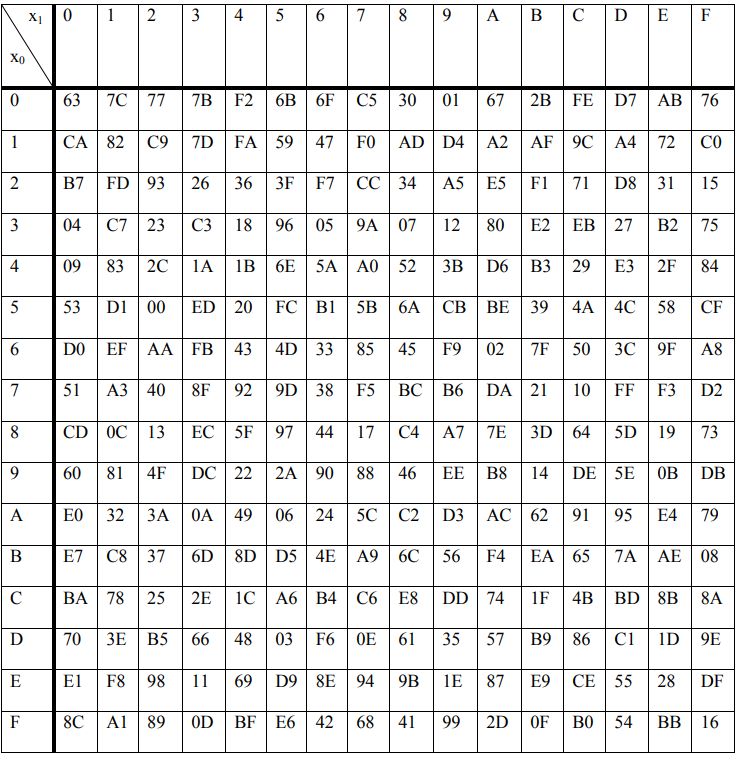
\includegraphics[width=0.5\linewidth]{SR.png} \\ Rijndael S-Box}
\end{figure}

    \begin{figure}[h!]
\center{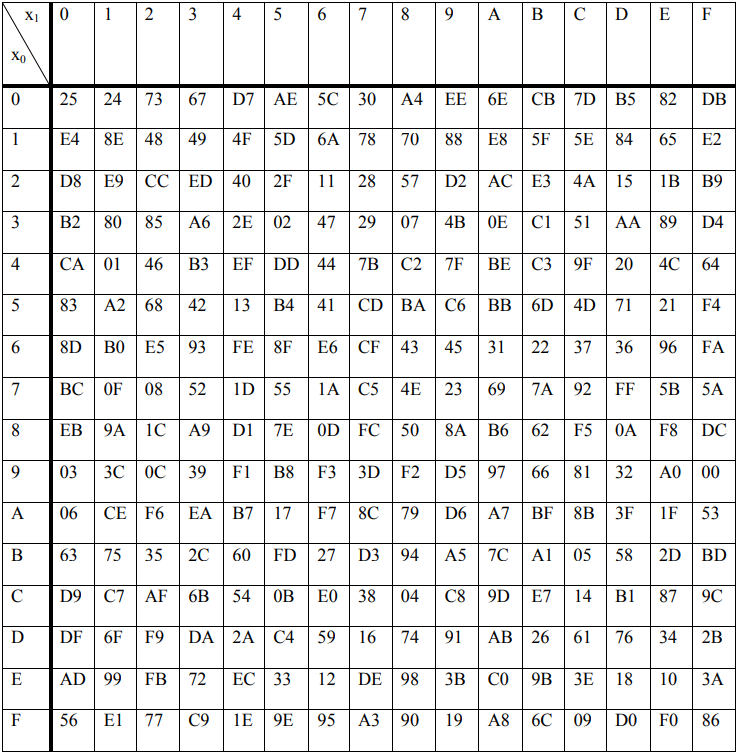
\includegraphics[width=0.5\linewidth]{SQ.png} \\ S-Box $S_Q$}
\end{figure}

    \item S-Box $S_1$
    Пусть 32-битное число $w$ представимо в виде $w = w_0 \mathbin\Vert w_1 \mathbin\Vert w_2 \mathbin\Vert w_3$. Тогда $S_1(w) = r_0 \mathbin\Vert r_1 \mathbin\Vert r_2 \mathbin\Vert r_3$, где:
    \begin{itemize}
        \item $r_0 = MULx(S_R(w_0), 0x1B) \oplus S_R(w_1) \oplus S_R(w_2) \oplus MULx(S_R(w_3), 0x1B) \oplus S_R(w_3)$;
        \item $r_1 = MULx(S_R(w_0), 0x1B) \oplus S_R(w_0) \oplus MULx(S_R(w_1), 0x1B) \oplus S_R(w_2) \oplus S_R(w_3)$;
        \item $r_2 = S_R(w_0)\oplus MULx(S_R(w_1), 0x1B) \oplus S_R(w_1) \oplus MULx(S_R(w_2), 0x1B) \oplus S_R(w_3)$;
        \item $r_3 = S_R(w_0) \oplus S_R(w_1) \oplus MULx(S_R(w_2), 0x1B) \oplus S_R(w_2) \oplus MULx(S_R(w_3), 0x1B)$.
    \end{itemize}
    
    \item S-Box $S_2$
    Пусть 32-битное число $w$ представимо в виде $w = w_0 \mathbin\Vert w_1 \mathbin\Vert w_2 \mathbin\Vert w_3$. Тогда $S_2(w) = r_0 \mathbin\Vert r_1 \mathbin\Vert r_2 \mathbin\Vert r_3$, где:
    \begin{itemize}
        \item $r_0 = MULx(S_Q(w_0), 0x69) \oplus S_Q(w_1) \oplus S_Q(w_2) \oplus MULx(S_Q(w_3), 0x69) \oplus S_Q(w_3)$;
        \item $r_1 = MULx(S_Q(w_0), 0x69) \oplus S_Q(w_0) \oplus MULx(S_Q(w_1), 0x69) \oplus S_Q(w_2) \oplus S_Q(w_3)$;
        \item $r_2 = S_Q(w_0)\oplus MULx(S_Q(w_1), 0x69) \oplus S_Q(w_1) \oplus MULx(S_Q(w_2), 0x69) \oplus S_Q(w_3)$;
        \item $r_3 = S_Q(w_0) \oplus S_Q(w_1) \oplus MULx(S_Q(w_2), 0x69) \oplus S_Q(w_2) \oplus MULx(S_Q(w_3), 0x69)$.
    \end{itemize}
    
\end{itemize}

Рассмотрим два основных режима работы шифра Snow3G:

\begin{itemize}
    \item Инициализация

Шифр инициализируется с использованием 128-битного ключа $k = k_0 \mathbin\Vert k_1 \mathbin\Vert k_2 \mathbin\Vert k_3$, состоящего из четырех 32-битных слов $k_0, k_1, k_2$ и $k_3$, а также с использованием 128-битного вектора инициализации $IV = IV_0 \mathbin\Vert IV_1 \mathbin\Vert IV_2 \mathbin\Vert IV_3$, также состоящего из четырех 32-битных слов $IV_0, IV_1, IV_2$ и $IV_3$. При этом с использованием данных параметров происходит инициализация содержимого ячеек регистра LFSR по следующим правилам:
\begin{longtable}{|p{2.5cm}|p{2.5cm}|p{2.5cm}|p{2.5cm}|}
\hline
$s_0 = k_0 \oplus 1^{32}$ & $s_1 = k_1 \oplus 1^{32}$ & $s_2 = k_2 \oplus 1^{32}$ & $s_3 = k_3 \oplus 1^{32}$ \\
\hline
$s_4 = k_0$ & $s_5 = k_1$ & $s_6 = k_2$ & $s_7 = k_3$ \\
\hline
$s_8 = k_0 \oplus 1^{32}$ & $s_9 = k_1 \oplus 1^{32} \oplus IV_3$ & $s_{10} = k_2 \oplus 1^{32} \oplus IV_2$ & $s_{11} = k_3 \oplus 1^{32}$ \\
\hline
$s_{12} = k_0 \oplus IV_1$ & $s_{13} = k_1$ & $s_{14} = k_2$ & $s_{15} = k_3 \oplus IV_0$ \\
\hline
\end{longtable}

Регистры $R_1, R_2$ и $R_3$ конечного автомата FSM инициализируются нулями: $R_1 = R_2 = R_3 = 0^{32}$.

Будем считать, что $s_0 = s_{0, 0} \mathbin\Vert s_{0, 1} \mathbin\Vert s_{0, 2} \mathbin\Vert s_{0, 3}$ и $s_{11} = s_{11, 0} \mathbin\Vert s_{11, 1} \mathbin\Vert s_{11, 2} \mathbin\Vert s_{11, 3}$. Генерации ключевого потока предшествуют следующие действия:

$For$ $t$ $=$ $1$ $to$ $32$ $do$ \{ 
    
    \hspace{0.5cm}$F = (s_{15} \boxplus R_1) \oplus R_2$;
    
    \hspace{0.5cm}$TEMP_1 = R_2 \boxplus (R_3 \oplus s_5)$;
    
    \hspace{0.5cm}$R_3 = S_2(R_2); R_2 = S_1(R_1); R_1 = TEMP_1$;

    \hspace{0.5cm}$TEMP_2 = (s_{0, 1} \mathbin\Vert s_{0, 2} \mathbin\Vert s_{0, 3} \mathbin\Vert 0x00) \oplus MUL_\alpha(s_{0, 0}) \oplus s_2 \oplus (0x00 \mathbin\Vert s_{11, 0} \mathbin\Vert s_{11, 1} \mathbin\Vert s_{11, 2}) \oplus DIV_\alpha(s_{11, 3}) \oplus F$;

    \hspace{0.5cm}$s_0~=~s_1;~s_1~=~s_2;~s_2~=~s_3;~s_3~=~s_4;~s_4~=~s_5;~s_5~=~s_6;~s_6~=~s_7;~s_7~=~s_8;~s_8~=~s_9$;
    
    \hspace{0.5cm}$s_9~=~s_{10};~s_{10}~=~s_{11};~s_{11}~=~s_{12};~s_{12}~=~s_{13};~s_{13}~=~s_{14};~s_{14}~=~s_{15};~s_{15}~=~TEMP_2$.
    
\}

Схема работы шифра при инициализации приведна ниже.
\begin{figure}[h!]
\center{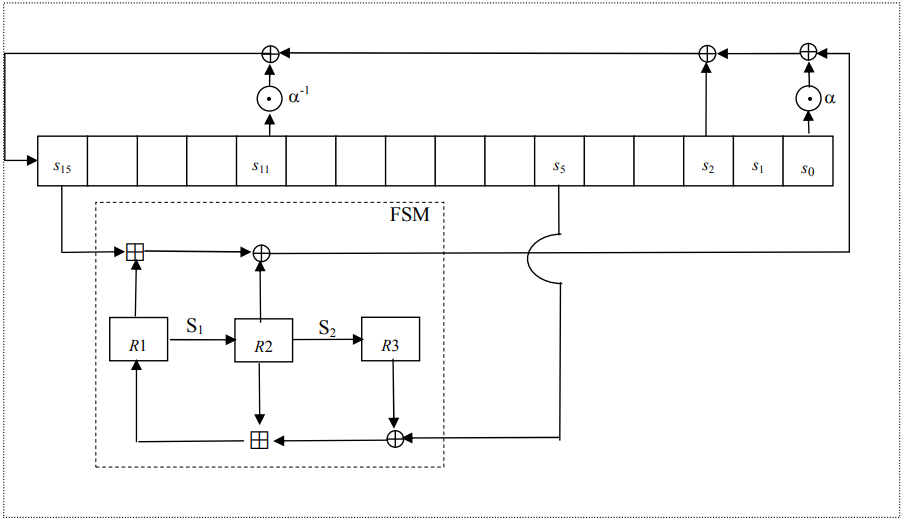
\includegraphics[width=0.7\linewidth]{snow_init.png} \\ Схема выполнения Snow3G при инициализации}
\end{figure}

\item Генерация ключевого потока

После инициализации для генерации $n$ 32-битных слов ключевого потока будут выполнены следующие действия:

$For$ $t$ $=$ $1$ $to$ $n$ $do$ \{ 
    
    \hspace{0.5cm}$F = (s_{15} \boxplus R_1) \oplus R_2$;
    
    \hspace{0.5cm}$TEMP_1 = R_2 \boxplus (R_3 \oplus s_5)$;
    
    \hspace{0.5cm}$R_3 = S_2(R_2); R_2 = S_1(R_1); R_1 = TEMP_1$;

    Одно 32-битное слово ключевого потока $z_t$ вычисляется следующим образом:

    \hspace{0.5cm}$z_t = F \oplus s_0$;

    \hspace{0.5cm}$TEMP_2 = (s_{0, 1} \mathbin\Vert s_{0, 2} \mathbin\Vert s_{0, 3} \mathbin\Vert 0x00) \oplus MUL_\alpha(s_{0, 0}) \oplus s_2 \oplus (0x00 \mathbin\Vert s_{11, 0} \mathbin\Vert s_{11, 1} \mathbin\Vert s_{11, 2}) \oplus DIV_\alpha(s_{11, 3}) \oplus F$;

    \hspace{0.5cm}$s_0~=~s_1;~s_1~=~s_2;~s_2~=~s_3;~s_3~=~s_4;~s_4~=~s_5;~s_5~=~s_6;~s_6~=~s_7;~s_7~=~s_8;~s_8~=~s_9$;
    
    \hspace{0.5cm}$s_9~=~s_{10};~s_{10}~=~s_{11};~s_{11}~=~s_{12};~s_{12}~=~s_{13};~s_{13}~=~s_{14};~s_{14}~=~s_{15};~s_{15}~=~TEMP_2$.

\}

Схема работы шифра при генерации ключевого потока приведна ниже.
\begin{figure}[h!]
\center{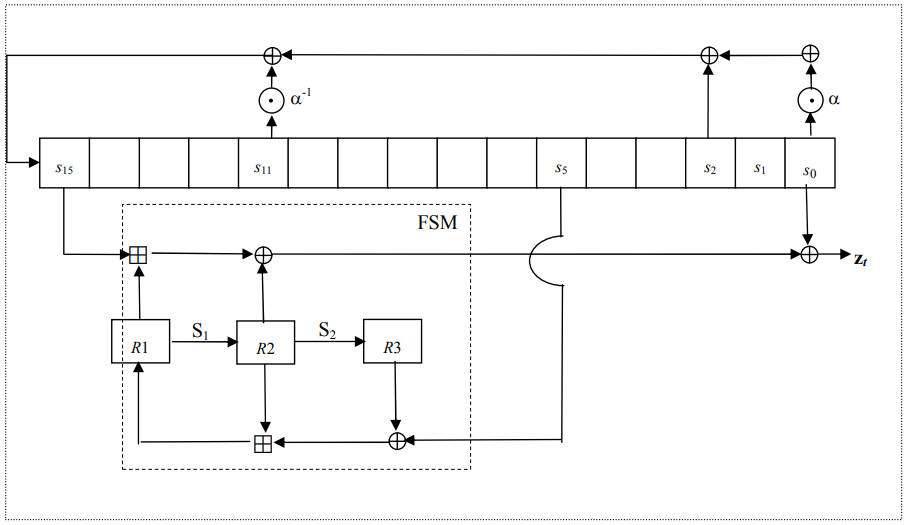
\includegraphics[width=0.7\linewidth]{snow_gen.png} \\ Схема выполнения Snow3G при генерации ключевого потока}
\end{figure}
    
\end{itemize}

\subsubsection{Анализ шифра}

В статье \cite{snow3g_2} устанавливаются оценки временной и пространственной сложностей компонентов шифра Snow3G. Справедливы следующие оценки:
\begin{itemize}
    \item Временная и пространственная сложности функций $MULx$, $MULxPOW$, $MUL_\alpha$, $DIV_\alpha$ равны $\textbf{O(1)}$;
    \item Временная и пространственная сложности S-блоков $S_1$, $S_2$ равны $\textbf{O(1)}$;
    \item Пусть $n$ --- число 32-битных слов ключевого потока, которые необходимо сгенерировать. Тогда временная сложность алгоритма Snow3G равна $\textbf{O(n)}$;
    \item Пространственная сложность алгоритма Snow3G равна $\textbf{O(1)}$.
\end{itemize}

Приведем описание некоторых атак на шифр Snow3G:
\begin{enumerate}
    \item
    Описание данной атаки приводится на основе работы \cite{atack1}.
    
    Для ключа $k$ случайным образом выбирается вектор инициализации $IV = IV_0 \mathbin\Vert IV_1 \mathbin\Vert IV_2 \mathbin\Vert IV_3$, по которому строится множество из 256 наборов, в котором варьируется старший байт $IV_0^0$ 32-битного слова $IV_0$: он принимает все значения от 0 до 255. Обозначим первое слово ключевого потока, сгенерированного на ключе $k$ и векторе инициализации $IV$, для которого $IV_0^0 = i$, $0 \leq i \leq 255$, через $z_{i, 0}$, а соответствующее содержимое в $j$-ой ячейке LFSR через $s_{i, j}$. Тогда: $\bigoplus_{i=0}^{255}{z_{i, 0}} = \bigoplus_{i=0}^{255}{(s_{i, 0} \oplus R_{i, 2})} \oplus \bigoplus_{i=0}^{255}{(s_{i, 15} \boxplus R_{i, 1})} = \bigoplus_{i=0}^{255}{(s_{i, 15} \boxplus R_{i, 1})}$. Показывается, что младший байт $\bigoplus_{i=0}^{255}{z_{i, 0}}$ всегда равен нулю. Это свойство подтверждается авторами экспериментально: авторами работы было выбрано $2^6$ векторов инициализации --- в каждом случае младший байт рассматриваемой суммы оказался равен нулю. Данное свойство представляет собой простую различительную атаку сложности $2^8$ по времени и по памяти для 13-раундового Snow3G.

    
    \item
    Описание данной атаки приводится на основе работы \cite{art4}.

    В данной статье производится сравнение линейных аппроксимаций шифра Snow3G, а также приводится описание атаки на основе использования линейной аппроксимации, направленной на восстановление секретного ключа. Для построения побитовой линейной аппроксимации конечного автомата используются следующие выражения: 

    \begin{itemize}
        \item $\Phi \cdot (z_{t-1} \oplus s_{t-1}) = \Phi \cdot (s_{t+14} \boxplus R_1^{t-1}) \oplus \Phi \cdot R_2^{t-1}$;
        \item $\Gamma \cdot (z_{t} \oplus s_{t}) = \Gamma \cdot (s_{t+15} \boxplus R_1^{t}) \oplus \Gamma \cdot R_2^{t}$;
        \item $\Lambda \cdot (z_{t+1} \oplus s_{t+1}) = \Lambda \cdot (s_{t+16} \boxplus R_1^{t+1}) \oplus \Lambda \cdot R_2^{t+1}$, где $\Phi, \Gamma, \Lambda$ --- некоторые 32-битные константы.
    \end{itemize}

    \begin{figure}[h!]
    \center{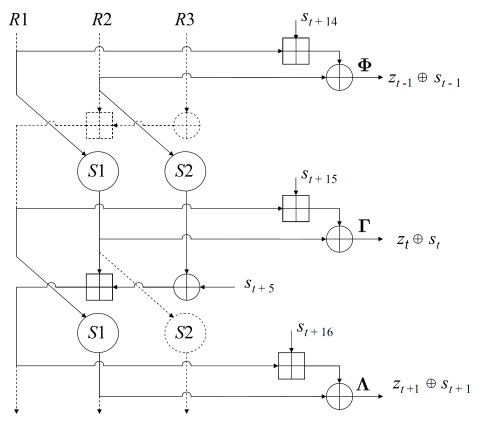
\includegraphics[width=0.5\linewidth]{aproksim.png} \\ Схема указанной линейной аппроксимации FSM}
    \end{figure}

    В результате преобразований система равенств, указанная выше, может быть приведена к виду: $\Phi \cdot z_{t-1} \oplus \Gamma \cdot z_t \oplus \Lambda \cdot z_{t+1} = \Phi \cdot (s_{t-1} \oplus s_{t+14}) \oplus \Gamma \cdot (s_t \oplus s_{t+15}) \oplus \Lambda \cdot (s_{t+1} \oplus s_{t+5} \oplus s_{t+16}) \oplus e^{(t)}$, где значения $e^{(t)}$ определяют двоичные шумы, вносимые побитовыми линейными аппроксимациями. В работе показывается, что наилучшее качество аппроксимации достигается на следующих наборах значений ($\Lambda, \Phi, \Gamma$): $\Lambda = 0x1014190f$, $\Phi = 0x00000020$, $\Gamma = 0x00000001$ и $\Lambda = 0x1014190f$, $\Phi = 0x00000030$, $\Gamma = 0x00000001$.

    На основе указанного выше представления описывается алгоритм, реализующий атаку, направленную на восстановление секретного ключа:

    Параметры алгоритма: $N$, $m_2$, $l (= 512)$, $l'$. 
    
    Вход алгоритма: слова $z_0, z_1, ..., z_{D-1}$, где $D = N/2 + 1$, ключевого потока, а также две тройки значений $(\Phi, \Gamma, \Lambda)$. 
    
    Генерально предложенный алгоритм состоит из следующих шагов:

    \begin{enumerate}
        \item Этап предварительной обработки с применением алгоритма $k$-дерева Вагнера (Wagner’s $k$-tree algorithm);
        \item Этап обработки --- восстановление $l'$ бит начального состояния LFSR с применением быстрого преобразования Уолша (FWT --- Fast Walsh Transform);
        \item Восстановление оставшихся $l - l'$ бит начального состояния LFSR;
        \item Восстановление секретного ключа путем выполнения действий в порядке, обратном инициализации.
    \end{enumerate}
    
    Сложности по времени и по памяти ограничены сверху значением $2^{174.16}$.

    \item 
    Описание данной атаки приводится на основе работы \cite{art5}. В данной работе описывается, в частности, различительная атака на Snow3G.

     Отметим, что преобразования, задаваемые S-блоками $S_1$ и $S_2$ могут быть определны следующим образом: $S_1(W) = L_1S_R(W)$, $S_2(W) = L_2S_Q(W)$, где $L_1, L_2$ определяются на основе таблиц S-блоков и являются невырожденными.
    
    $z^{t-1} = (S_R^{-1}(L_1^{-1}R_2^{t}) \boxplus s_{15}^{t-1}) \oplus S_Q^{-1}(L_2^{-1}R_3^{t}) \boxplus s_0^{t-1}$;

    Рассматривается следующая схема аппроксимации (через $X[0]$ обозначен нулевой байт 32-битного слова $X$):
    \begin{itemize}
        \item $z^{t-1}[0] = n_0 \oplus (s_{15}^{t-1} \oplus s_0^{t-1})[0]$;
        \item $z^{t}[0] = n_1 \oplus (s_{15}^{t} \oplus s_0^{t})[0]$;
        \item $L_1^{-1}z^{t+1}[0] = n_2 \oplus (L_1^{-1}s_5^{t} \oplus L_1^{-1}s_{15}^{t+1} \oplus L_1^{-1}s_0^{t+1})[0]$.
    \end{itemize}

    Убирая вклад LFSR, получаем: $S^t = ((s_{15}^{t-1} \oplus s_0^{t-1})[0], (s_{15}^{t} \oplus s_0^{t})[0], (L_1^{-1}s_{15}^{t+1} \oplus L_1^{-1}s_0^{t+1})[0])$.

    Авторами доказывается тот факт, что если существуют такие $t_1, t_2, t_3$, что $s_0^0 \oplus s_0^{t_1} \oplus s_0^{t_2} \oplus s_0^{t_3} = 0$, то $S^t \oplus S^{t + t_1} \oplus S^{t + t_2} \oplus S^{t + t_3} = (0, 0, 0)$.

    В предположении, что такие $t_1, t_2, t_3$ найдены, можно составить следующие выборки: \\ $x^t = \sum_{i=0}^{3}(z^{t+t_i-1}[0], z^{t+t_i}[0], L_1^{-1}z^{t+t_i+1}[0])$, где $t_0 = 0$, которые используются для различения последовательности от истинно случайной. Для решения задачи нахождения необходимых $t_1, t_2, t_3$ используется представленный в статье \cite{temp} алгоритм.

    Авторами показано, что требуется порядка $2^{163}$ символов ключевого потока, чтобы отличить выборки от истинно случайных.

    Сложности по времени и по памяти равны примерно $2^{172}$.
    
\end{enumerate}

В работе \cite{art2} описываются результаты статистического тестирования шифра Snow3G с использованием набора статистических тестов NIST, в который входят следующие тесты: частотный побитовый тест, частотный блочный тест, тест на последовательность одинаковых битов, тест на самую длинную серию единиц в блоке, тест ранга двоичной матрицы, тест дискретного преобразования Фурье (спектральный), тест на совпадение неперекрывающихся шаблонов, тест на совпадение перекрывающихся шаблонов, универсальный статистический тест Маурера, тест на линейную сложность, тест на периодичность, тест приблизительной энтропии, тест кумулятивных сумм, тест случайного отклонения, другой тест случайного отклонения. Указанные тесты были применены для оценки случайности длинного ключевого потока (для каждого из 300 случайно выбранных ключей генерировалось $2^{20}$ бит ключевого потока, IV нулевой), для оценки случайности короткого ключевого потока (для каждого из 307200 случайно выбранных ключей генерировалось $2^{10}$ бит ключевого потока, IV нулевой), для оценки корреляции между различными значениями IV (генерируются 300 наборов данных из случайно выбранных ключей; каждый набор представляет собой объединение 256 последовательностей длиной 4096 бит каждая; первая последовательность генерируется с нулевым IV, каждая последующая --- с увеличивающимся на 1 значением IV).

Шифром были успешно пройдены все тесты оценки случайности длинного ключевого потока и оценки корреляции между различными значениями IV --- тесты не выявили отклонений от истинно случайных последовательностей. При этом для набора данных для оценки случайности короткого ключевого потока шифром не было пройдено 8 тестов: тест на последовательность одинаковых битов, тест на самую длинную серию единиц в блоке, тест ранга двоичной матрицы, тест дискретного преобразования Фурье, тест на совпадение неперекрывающихся шаблонов, тест на совпадение перекрывающихся шаблонов, тест приблизительной энтропии, тест на периодичность --- на тестах допускается возможность отличить первые 1024 бита ключевого потока от истинно случайной последовательности.

В работе \cite{art1} исследуются различные подходы к программной реализации шифра Snow3G на двух основных платформах мобильных телефонов. Авторами работы были подготовлены реализации шифра для платформы iOS с использованием языка программирования Objective-C, а также для платформы Android с использованием языка программирования Java. 

\begin{longtable}{|p{1cm}|p{1cm}|p{1cm}|p{1cm}|p{1cm}|p{1cm}|p{1cm}|p{1cm}|p{1cm}|p{1cm}|}
\hline
\multicolumn{2}{|c|}{Traditional} & \multicolumn{2}{c|}{HardCode} & \multicolumn{2}{c|}{Circular Buffers} & \multicolumn{2}{c|}{Sliding Windows} & \multicolumn{2}{c|}{Loop Unrolling} \\
\hline
\multicolumn{2}{|c|}{Time (ms)} & \multicolumn{2}{c|}{Time (ms)} & \multicolumn{2}{c|}{Time (ms)} & \multicolumn{2}{c|}{Time (ms)} & \multicolumn{2}{c|}{Time (ms)} \\
\hline
iOS & Android & iOS & Android & iOS & Android & iOS & Android & iOS & Android \\
\hline
491.1 & 1772.05 & 342.5 & 1513.97 & 834 & 1057.719 & 184.1 & 943.569 & 291.3 & 1697.843 \\
\hline
\end{longtable}

В данной работе рассматриваются различные методы реализации сдвига LFSR для минимизации времени работы щифра. Для каждого метода производились замеры времени генерации $10^7$ байт ключевой последовательности в целом, а также замеры отводимого при этом времени на сдвиги содержимого LFSR. Результаты тестирования приведены в таблице ниже. Лучшей по времени выполнения оказалась реализация LFSR с использованием метода скользящих окон (Sliding Windows). В данной реализации размер регистра LFSR увеличивается в 2 раза, его содержимое дублируется во второй половине. Используется один указатель, изначально указывающий на начало второй половины регистра; при достижении конца регистра он возвращается в исходное положение. Вычисляемое новое значение записывается в первой позиции окна и в позиции, на которую указывает указатель. После этого окно (указатель) сдвигается на одну позицию.

В статье \cite{art3} описывается эффективная аппаратная реализация шифра Snow3G с использованием ASIC.

\begin{figure}[h]
\center{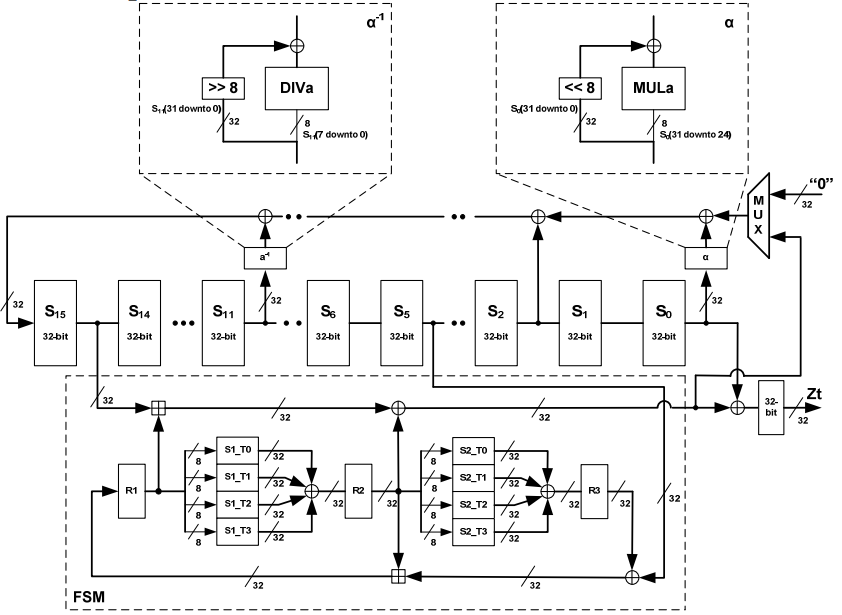
\includegraphics[width=0.8\linewidth]{arch} \\ Предлагаемая авторами \cite{art3} подробная архитектура аппаратной реализации Snow3G}
\end{figure}

Для вычисления значений S-блоков предлагается использовать специальные таблицы $S1\_T0, S1\_T1, S1\_T2, S1\_T3$ и $S2\_T0, S2\_T1, S2\_T2, S2\_T3$: для $w = w_0 \mathbin\Vert w_1 \mathbin\Vert w_2 \mathbin\Vert w_3$ $S_1(w) = S1\_T0(w_3)\oplus S1\_T1(w_2) \oplus S1\_T2(w_1) \oplus S1\_T3(w_0)$, $S_2(w) = S2\_T0(w_3) \oplus S2\_T1(w_2) \oplus S2\_T2(w_1) \oplus S2\_T3(w_0)$. Через мультиплексор (MUX) происходит выбор режима работы Snow3G: инициализация или генерация ключевой последовательности. Операция сложения по модулю $2^{32}$ реализована с помощью сумматоров с ускоренным переносом. Функции $MUL_\alpha$ и $DIV_\alpha$ реализованы с помощью некоторых таблиц $MUL_{alpha}$ и $DIV_{alpha}$ соответственно. 

Аппаратная реализация состояла из 25016 вентилей, критический путь составил 4.03 нс. На тестах было показано, что предложенная авторами реализация позволяет достичь максимальной частоты в 249 МГц, и максимального значения пропускной способности в 7968 Мбит/с, хоть и является менее компактной по сравнению с другими аппаратными реализациями других поточных шифров.

\subsection{Шифр LILI128}

Описание шифра LILI128 приводится в соответствии с описанием, представленным в работе \cite{lili} разработчиков данного шифра.

Генератор состоит из двух регистров сдвига с линейной обратной связью $LFSR_c$ и $LFSR_d$, состоящих из 39 и 89 битовых ячеек памяти соответственно. Кроме того, для генерации ключевого потока используются две функции: $f_c$ и $f_d$, которые описываются далее. Функционально генератор может быть разделен на две подсистемы: подсистема управления тактами (Clock-Control Subsystem) и подсистема генерации данных (Data Generation Subsystem).

При инициализации генератора используется 128-битный ключ, первыми 39 битами которого инициализируется регистр $LFSR_c$, а оставшимися 89 --- регистр $LFSR_d$.


Характеристики подсистемы управления тактами:
\begin{itemize}
    \item Используется для генерации псевдослучайной последовательности $c = \{c(t)\}_{t = 1}^{\infty}$. В момент времени $t$ значением $c(t)$ определяется количество тактов, которое необходимо сделать регистру $LFSR_d$ подсистемы генерации данных перед генерацией очередного бита $z(t)$ ключевого потока;
    \item Полином обратной связи для регистра $LFSR_c$ имеет следующий вид: $x^{39} + x^{35} + x^{33} + x^{31} + x^{17} + x^{15} + x^{14} + x^2 + x + 1$;
    \item Функция $f_c: \mathbb{F}^2_2 \rightarrow \{ 1, 2, 3, 4 \}$ зависит от двух параметров и имеет следующий вид: $f(x_{12}, x_{20}) = 2x_{12} + x_{20} + 1$.
\end{itemize}

Характеристики подсистемы генерации данных:
\begin{itemize}
    \item Используется для генерации псевдослучайной последовательности $z = \{z(t)\}_{t = 1}^{\infty}$, составляющией ключевой поток;
    \item Полином обратной связи для регистра $LFSR_d$ имеет следующий вид: $x^{89} + x^{83} + x^{80} + x^{55} + x^{53} + x^{42} + x^{39} + x + 1$;
    \item Функция $f_d: \mathbb{F}^{10}_2 \rightarrow \mathbb{F}_2$ задается своей таблицей истинности. Вектор значений функции длины 1024 задается следующим образом:

\begin{longtable}{|p{7.5cm}|}
\hline
0,0,1,1,1,1,0,0,1,1,0,0,0,0,1,1,1,1,0,0,0,0,1,1,0,0,1,1,1,1,0,0, \\
0,0,1,1,1,1,0,0,1,1,0,0,0,0,1,1,1,1,0,0,0,0,1,1,0,0,1,1,1,1,0,0, \\
0,0,1,1,1,1,0,0,1,1,0,0,0,0,1,1,1,1,0,0,0,0,1,1,0,0,1,1,1,1,0,0, \\
1,1,0,0,0,0,1,1,0,0,1,1,1,1,0,0,0,0,1,1,1,1,0,0,1,1,0,0,0,0,1,1, \\
0,1,0,1,1,0,1,0,1,0,1,0,0,1,0,1,1,0,1,0,0,1,0,1,0,1,0,1,1,0,1,0, \\
0,1,0,1,1,0,1,0,1,0,1,0,0,1,0,1,1,0,1,0,0,1,0,1,0,1,0,1,1,0,1,0, \\
0,1,0,1,1,0,1,0,1,0,1,0,0,1,0,1,1,0,1,0,0,1,0,1,0,1,0,1,1,0,1,0, \\
1,0,1,0,0,1,0,1,0,1,0,1,1,0,1,0,0,1,0,1,1,0,1,0,1,0,1,0,0,1,0,1, \\
0,1,1,0,0,1,1,0,1,0,0,1,1,0,0,1,1,0,0,1,1,0,0,1,0,1,1,0,0,1,1,0, \\
0,1,1,0,0,1,1,0,1,0,0,1,1,0,0,1,1,0,0,1,1,0,0,1,0,1,1,0,0,1,1,0, \\
0,1,1,0,1,0,0,1,0,1,1,0,1,0,0,1,1,0,0,1,0,1,1,0,1,0,0,1,0,1,1,0, \\
0,1,1,0,1,0,0,1,1,0,0,1,0,1,1,0,0,1,1,0,1,0,0,1,1,0,0,1,0,1,1,0, \\
0,0,0,0,1,1,1,1,1,1,1,1,0,0,0,0,1,1,1,1,0,0,0,0,0,0,0,0,1,1,1,1, \\
1,1,1,1,0,0,0,0,0,0,0,0,1,1,1,1,0,0,0,0,1,1,1,1,1,1,1,1,0,0,0,0, \\
0,0,1,1,0,0,1,1,1,1,0,0,1,1,0,0,1,1,0,0,1,1,0,0,0,0,1,1,0,0,1,1, \\
1,1,0,0,1,1,0,0,0,0,1,1,0,0,1,1,0,0,1,1,0,0,1,1,1,1,0,0,1,1,0,0, \\
0,0,1,1,1,1,0,0,0,0,1,1,1,1,0,0,1,1,0,0,0,0,1,1,1,1,0,0,0,0,1,1, \\
1,1,0,0,0,0,1,1,1,1,0,0,0,0,1,1,0,0,1,1,1,1,0,0,0,0,1,1,1,1,0,0, \\
0,0,1,1,1,1,0,0,1,1,0,0,0,0,1,1,0,0,1,1,1,1,0,0,1,1,0,0,0,0,1,1, \\
1,1,0,0,0,0,1,1,0,0,1,1,1,1,0,0,1,1,0,0,0,0,1,1,0,0,1,1,1,1,0,0, \\
0,1,0,1,0,1,0,1,1,0,1,0,1,0,1,0,1,0,1,0,1,0,1,0,0,1,0,1,0,1,0,1, \\
1,0,1,0,1,0,1,0,0,1,0,1,0,1,0,1,0,1,0,1,0,1,0,1,1,0,1,0,1,0,1,0, \\
0,1,0,1,1,0,1,0,0,1,0,1,1,0,1,0,1,0,1,0,0,1,0,1,1,0,1,0,0,1,0,1, \\
1,0,1,0,0,1,0,1,1,0,1,0,0,1,0,1,0,1,0,1,1,0,1,0,0,1,0,1,1,0,1,0, \\
0,1,0,1,1,0,1,0,1,0,1,0,0,1,0,1,0,1,0,1,1,0,1,0,1,0,1,0,0,1,0,1, \\
1,0,1,0,0,1,0,1,0,1,0,1,1,0,1,0,1,0,1,0,0,1,0,1,0,1,0,1,1,0,1,0, \\
0,1,1,0,0,1,1,0,0,1,1,0,0,1,1,0,1,0,0,1,1,0,0,1,1,0,0,1,1,0,0,1, \\
1,0,0,1,1,0,0,1,1,0,0,1,1,0,0,1,0,1,1,0,0,1,1,0,0,1,1,0,0,1,1,0, \\
0,1,1,0,0,1,1,0,1,0,0,1,1,0,0,1,0,1,1,0,0,1,1,0,1,0,0,1,1,0,0,1, \\
1,0,0,1,1,0,0,1,0,1,1,0,0,1,1,0,1,0,0,1,1,0,0,1,0,1,1,0,0,1,1,0, \\
0,1,1,0,1,0,0,1,0,1,1,0,1,0,0,1,0,1,1,0,1,0,0,1,0,1,1,0,1,0,0,1, \\
1,0,0,1,0,1,1,0,1,0,0,1,0,1,1,0,1,0,0,1,0,1,1,0,1,0,0,1,0,1,1,0 \\
\hline
\end{longtable}
\end{itemize}

Генерация очередного бита $z(t)$ ключевого потока происходит по следущей процедуре:
\begin{enumerate}
    \item На вход функции $f_d$ подается $n~=~10$ битов регистра $LFSR_d$ --- биты под номерами 0, 1, 3, 7, 12, 20, 30, 44, 65, 80, в результате чего функцией $f_d$ возвращается бит $z(t)$ ключевого потока.
    \item На вход функции $f_c$ подается $k = 2$ бита регистра $LFSR_c$ --- биты под номерами 12 и 20, в результате чего функцией $f_c$ возвращается величина количиства сдвигов $c(t)$.
    \item Происходит один сдвиг содержимого регистра $LFSR_c$ и $c(t)$ (от 1 до 4) сдвигов содержимого регистра $LFSR_d$.
\end{enumerate}

\begin{figure}[h]
\center{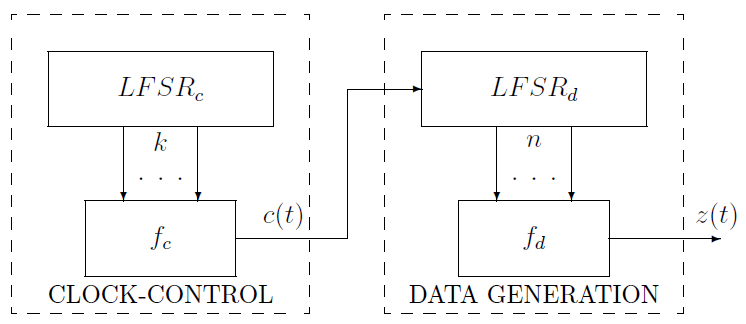
\includegraphics[width=0.5\linewidth]{lili128} \\ Схема генератора $LILI128$}
\end{figure}

\subsection{Шифр SEAL}
Приведем определение шифра SEAL согласно статье \cite{seal} авторов данного шифра.

В шифре используются 160-битный ключ $a$, 32-битная строка $n$ и длину генерируемой последовательности $L$. Выполнение шифра может быть разделено на две стадии: подготовка необходимых таблиц и непосредственно генерация ключевой последовательности.

Стадия 1 --- подготовка вспомогательных таблиц.
При шифровании используются значения трех таблиц: $R$, $S$ и $T$, содержимое которых определяется значением ключа $a$. Для заполнения данных таблиц предназначена функция $\Gamma$.

Функция $\Gamma$ определяется через функцию $G$, которая для 160-битной строки $a$ и 32-битного числа $i$ возвращает 160-битное значение $G_a(i)$.

Для описания функции $G$ необходимо определить при различных целочисленных значениях $0 \leq t \leq 79$ шестнадцатиричные константы $K_t$ и булевы функции $f_t$ следующим образом:
\begin{itemize}
    \item Для $0 \leq t \leq 19$: $K_t = 0x5A827999$ и $f_t(B, C, D) = (B \& C) \vee (\bar B \& D)$;
    \item Для $20 \leq t \leq 39$: $K_t = 0x6ED9EBA1$ и $f_t(B, C, D) = B \oplus C \oplus D$;
    \item Для $40 \leq t \leq 59$: $K_t = 0x8F1BBCDC$ и $f_t(B, C, D) = (B \& C) \vee (B \& D) \vee (C \& D)$;
    \item Для $60 \leq t \leq 79$: $K_t = 0xCA62C1D6$ и $f_t(B, C, D) = B \oplus C \oplus D$.
\end{itemize}

Будем рассматривать входную строку $a$ как последовательность из пяти 32-битных слов: $a = H_0\mathbin\Vert H_1 \mathbin\Vert H_2 \mathbin\Vert H_3 \mathbin\Vert H_4$. Также определим 512-битное слово $M = i \mathbin\Vert 0^{480}$, которое разобьем на 16 последовательных 32-битных слов: $M_0 = i$, $M_1 = M_2 = ... = M_{15} = 0$. После этого выполняется следующий алгоритм, в результате которого вычисляется значение $G_a(i)$:
\begin{enumerate}
    \item $For$ $t$ $=$ $16$ $to$ $79$ $do$ \{ 
    
    \hspace{0.5cm}$W_t = (W_{t-3} \oplus W_{t-8} \oplus W_{t-14} \oplus W_{t-16}) << 1$;
    
    \}
    \item Определим $A = H_0$, $B = H_1$, $C = H_2$, $D = H_3$, $E = H_4$;
    \item $For$ $t$ $=$ $16$ $to$ $79$ $do$ \{
    
    \hspace{0.5cm}$TEMP = (A << 5)$ + $f_t(B, C, D)$ + $E$ + $W_t$ + $K_t$;
    
    \hspace{0.5cm}$E = D;$ $D = C;$ $C = B << 30;$ $B = A;$ $A = TEMP;$
    
    \}
    \item $H_0 = H_0 + A;$ $H_1 = H_1 + B;$ $H_2 = H_2 + C;$ $H_3 = H_3 + D;$ $H_4 = H_4 + E$;
    \item $G_a(i)$ = $H_0 \mathbin\Vert H_1 \mathbin\Vert H_2 \mathbin\Vert H_3 \mathbin\Vert H_4$.
\end{enumerate}

Введем функцию $\Gamma$: $\Gamma_a(i)$ $=$ $H_{i~mod~5}^i$, где $H_0^{5j} \mathbin\Vert  H_1^{5j + 1} \mathbin\Vert H_2^{5j + 2} \mathbin\Vert H_3^{5j + 3} \mathbin\Vert H_4^{5j + 4}$ $=$ $G_a(j)$, $j = \lfloor i/5 \rfloor$. Значения, возвращаемые функцией $\Gamma$, используются для формирования таблиц $R$, $S$, $T$ по следующим правилам:
\begin{itemize}
    \item $T[i]~=~\Gamma_a(i)$, где $0 \leq i < 512$;
    \item $S[j]~=~\Gamma_a(0x1000 + j)$, где $0 \leq j < 256$;
    \item $R[k]~=~\Gamma_a(0x2000 + k)$, где $0 \leq k < 256$.
\end{itemize}

Кроме того, для генерации ключевого потока необходима функция инициализации $Initialize$. На вход данной функции подаются параметр $n$, являющийся входным параметром данного шифра, некоторое число $l$, четыре регистра $A, B, C, D$ и четыре 32-битных слова $n_1, n_2, n_3, n_4$. Тело функции имеет следующий вид:
\begin{figure}[h]
\center{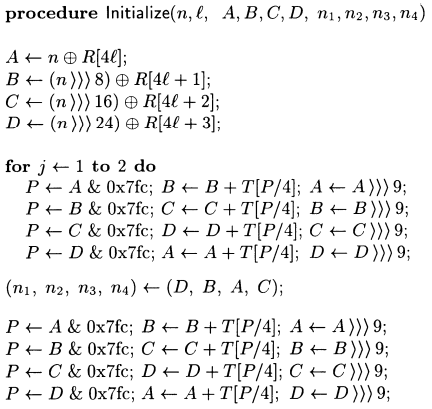
\includegraphics[width=0.5\linewidth]{image} \\ Функция $Initialize$}
\end{figure}

В результате работы функции $Initialize$, используя значения таблиц $R$ и $T$, инициализируются значениями регистры $A, B, C$ и $D$, а также переменные $n_1, n_2, n_3$ и $n_4$.

Стадия 2 --- генерация ключевого потока.
Для генерации непосредственно ключевого потока используется псевдослучайная функция $SEAL$. На вход данной функции поступают 160-битный ключ $a$, 32-битная строка $n$ и значение длины генерируемой последовательности $L$. Значение $L$ может быть настолько большим или настолько малым, насколько это необходимо для целевого приложения, но ожидаемая длина выходных данных составляет от нескольких байт до нескольких тысяч байт.

На каждом новом шаге для генерации ключевой последовательности функцией $SEAL$ вызывается функция $Initialize$ со значением $l$, равным номеру теущего шага. Генерация функцией $SEAL$ ключевого потока на очередной итерации происходит следующим образом: 
\begin{enumerate}
    \item На очередной итерации с использованием содержимого одного из регистров $A, B, C, D$ (9 старших битов) выбирается значение таблицы $T$. Выбранное значение складывается с находящимся в регистре $B, C, D, A$ значением соответственно;
    \item Содержимое регистра, использовавшегося для получения значения талицы $T$, сдвигается циклически вправо на 9 позиций;
    \item Содержимое регистра, с содержимым которого складывалось значение таблицы $T$, складывается с содержимым сдвинутого на шаге 2 регистра, либо не изменяется;
    \item Значения регистров $A, B, C, D$ складываются со значениями таблицы $S$, определяемыми номером текущей итерации. Полученное значение добавляется в ключевую последовательность;
    \item Если длина сгенерированной к данному моменту ключевой последовательности превышает заданное значение $L$, то функция возвращает элементы $0, ..., (L-1)$ ключевой последовательности;
    \item К содержимому регистров $A, B, C, D$ прибавляются значения $n_1, n_2, n_3, n_4$.
\end{enumerate}
Для очередного значения $l$ может быть выполнено 64 итерации генерации элементов ключевой последовательности. Если за 64 итерации длина сгенерированной ключевой последовательности меньше $L$, то происходит переход к следующему шагу: увеличивается знаечение $l$.

\begin{figure}[h]
\center{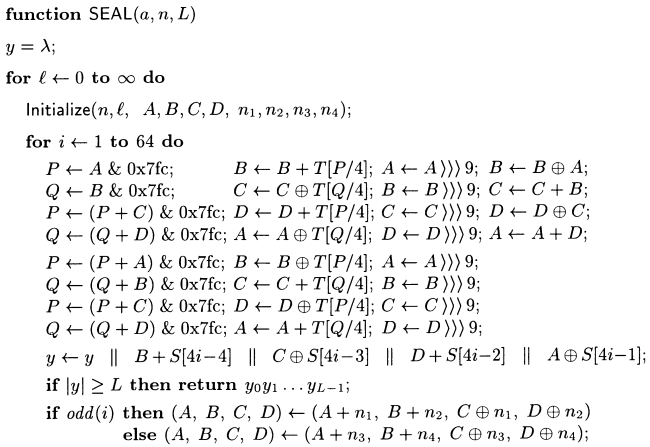
\includegraphics[width=0.7\linewidth]{image2} \\ Функция $SEAL$}
\end{figure}

\subsection{Шифр MUGI}
Далее приводится описание шифра MUGI, следуя статье \cite{mugi} разработчиков данного шифра.

На вход шифру подается 128-битный секретный ключ $K = K_0 \mathbin\Vert K_1$, старшие 64 бита которого обозначим через $K_0$, а оставшиеся --- через $K_1$, и 128-битный публичный вектор инициализации $IV = IV_0 \mathbin\Vert IV_1$, старшие 64 бита которого обозначим через $IV_0$, а оставшиеся --- через $IV_1$.

Для функционирования MUGI определяется внутреннее состояние, включающее в себя:
\begin{itemize}
    \item состояние $a$: три 64-битных регистра состояния ($a_0, a_1, a_2$);
    \item буфер $b$: шестнадцать 64-битных буферных регистра ($b_0, b_1, ..., b_{15}$).
\end{itemize}
В каждый момент времени $t$ внутреннее состояние содержит некоторые значения: $a^{(t)} = (a_0^{(t)}, a_1^{(t)}, a_2^{(t)})$ и \\ $b^{(t)} = (b_0^{(t)}, b_1^{(t)}, ..., b_{15}^{(t)})$. Для обновления состояния $a$ предназначена функция $\rho$, для обновления буфера $b$ --- функция $\lambda$. Таким образом, обновление внутреннего состояния описывается следующим образом: \\ $(a^{(t+1)}, b^{(t+1)}) = (\rho(a^{(t)}, b^{(t)}), \lambda(a^{(t)}, b^{(t)})) = \Upsilon(a^{(t)}, b^{(t)})$.


Выполняемые функцией $\rho$ действия при вызове $\rho(a^{(t)}, b^{(t)})$:
\begin{itemize}
    \item $a_0^{(t+1)} = a_1^{(t)}$;
    \item $a_1^{(t+1)} = a_2^{(t)} \oplus F(a_1^{(t)}, b_4^{(t)}) \oplus C_1$, где $C_1 = 0xBB67AE8584CAA73B$;
    \item $a_2^{(t+1)} = a_0^{(t)} \oplus F(a_1^{(t)}, b_{10}^{(t)} <<< 17) \oplus C_2$, где $C_2 = 0x3C6EF372FE94F82B$.
\end{itemize}

Выполняемые функцией $\lambda$ действия при вызове $\lambda(a^{(t)}, b^{(t)})$:
\begin{itemize}
    \item $b_j^{(t+1)} = b_{j-1}^{(t)}$, где $j \neq 0, 4, 10$;
    \item $b_0^{(t+1)} = b_{15}^{(t)} + a_0^{(t)}$;
    \item $b_4^{(t+1)} = b_3^{(t)} + b_7^{(t)}$;
    \item $b_{10}^{(t+1)} = b_9^{(t)} \oplus (b_{13}^{(t)} <<< 32)$.
\end{itemize}

Опишем выполняемые при инициализации действия (через $t_0$ обозначен момент начала инициализации):

Инициализация содержимого состояния $a$: $a_0^{(t_0)} = K_0$, $a_1^{(t_0)} = K_1$, $a_2^{(t_0)} = (K_0 <<< 7) \oplus (K_1 >>> 7) \oplus C_0$, где $C_0 = 0x6A09E667F3BCC908$.

После этого происходит инициализации содержимого буфера $b$ с использованием значений регистра $a_0$: $b_{15-i} = (\rho^{(i + 1)}(a^{(t_0)}, 0))_0$, где $0 \leq i \leq 15$.

Введем обозначения: $a(K) = \rho^{16}(a^{(t_0)}, 0)$, $a(K, IV)_0 = a(K)_0 \oplus IV_0$, $a(K, IV)_1 = a(K)_1 \oplus IV_1$, $a(K, IV)_2 = a(K)_2 \oplus (IV_0 <<< 7) \oplus (IV_1 >>> 7) \oplus C_0$. Затем ещё раз происходит обновление состояния $a$ вызовом $\rho^{16}(a(K, IV), 0)$.

Завершающий этап инициализации: $a^{(1)} = \Upsilon^{16}(\rho^{16}(a(K, IV), 0), b(K))$, где через $b(K)$ обозначен инициализированный ранее секретным ключом $K$ буфер $b$. После этого содержимое внутреннего состояния определяется в результате выполнения описанной ранее функции $\Upsilon$.

Сгенерированным в момент времени $t$ словом ключевого потока считается 64-битное значение регистра $a_2$: \\ $z_t = a_2^{(t)}$.

\subsection{Шифры семейства A5}
Описания алгоритмов не были опубликованы консорциумом GSM.
Описания шифров A5/1, A5/2 и A5/3 приводятся согласно работам \cite{a5_1}, \cite{a5_2}.

\subsubsection{Шифр A5/1}
Шифр A5/1 состоит из трех регистров сдвига с линейной обратной связью:
\begin{enumerate}
    \item 19-битный регистр $R_1$, полином обратной связи которого имеет следующий вид: $x^{19} + x^{5} + x^{2} + x + 1$;
    \item 22-битный регистр $R_2$, полином обратной связи которого имеет следующий вид: $x^{22} + x + 1$;
    \item 23-битный регистр $R_3$, полином обратной связи которого имеет следующий вид: $x^{23} + x^{15} + x^{2} + x + 1$.
\end{enumerate}
Кроме того, имеется механизм управления тактированием:
для управления ... в каждом регистре выбрано по одному специальному биту, называемому битом синхронизации: для регистра $R1$ --- 8, для регистров $R_2$ и $R_3$ --- 10. С использованием значений указанных битов вычисляется значение функции $f(x, y, z) = (x \& y) \vee (x \& z) \vee (y \& z)$, где $x, y, z$ --- значения битов синхронизации регистров $R_1, R_2, R_3$ соответственно. После вычисления значения $f(x, y, z)$ происходит сдвиг только тех регистров, бит синхронизации которых равен $f(x, y, z)$.

Инициализация. На вход функции инициализации передются секретный 64-битный ключ $Key$ и 22-битный номер фрейма $Frame$ (в GSM системах в качестве единицы передаваемой информации используется фрейм, состоящий из 228 бит). Процедура инициализации состоит из следующих шагов: 
\begin{enumerate}
    \item $R_1 = 0^{19}$, $R_2 = 0^{22}$, $R_3 = 0^{23}$;
    \item $For~i~=~0~to~63~do~\{$
    
    \hspace{0.5cm}Сложение по модулю $2$ младших битов (битов на нулевой позиции) регистров $R_1, R_2$ и $R_3$ cо значением $Key[i]$;

    \hspace{0.5cm}Сдвиг содержимого всех трех регистров;

    \}
    \item $For~i~=~0~to~21~do~\{$

    \hspace{0.5cm}Сложение по модулю $2$ младших битов (битов на нулевой позиции) регистров $R_1, R_2$ и $R_3$ cо значением $Frame[i]$;

    \hspace{0.5cm}Сдвиг содержимого всех трех регистров;

    \}
    \item $For~i~=~0~to~99~do~\{$

    \hspace{0.5cm}Сдвиги содержимого регистров $R_1, R_2, R_3$ с использованием механизма управления тактированием.

    \}
\end{enumerate}

Генерация ключевой последовательности. Элементом ключевой последовательности после выполнения очередного такта является сумма по модулю два выходных битов регистров.
После выполнения функции инициализации выполняется 228 тактов работы генератора, в результате чего формируется ключевая последовательность. Затем номер фрейма увеличивается на единицу, повторяются процессы инициализации и генерации ключевого потока.

\subsubsection{Шифр A5/2}
Шифр A5/2 также состоит из описанных ранее регистров $R_1, R_2, R_3$ и дополнительного 17-битного регистра сдвига с линейной обратной связью $R_4$, полином обратной связи которого имеет вид: $x^{17} + x^5 + 1$. Также присутствует механизм тактирования, главной частью которого является регистр $R_4$: для сдвига регистров вычисляется функция $f(x, y, z) = (x \& y) \vee (x \& z) \vee (y \& z)$ от 3, 7 и 10 битов регистра $R_4$, после чего:
\begin{itemize}
    \item регистр $R_1$ сдвигается, если значение 10 бита $R_4$ равно $f(x, y, z)$;
    \item регистр $R_2$ сдвигается, если значение 3 бита $R_4$ равно $f(x, y, z)$;
    \item регистр $R_3$ сдвигается, если значение 7 бита $R_4$ равно $f(x, y, z)$.
\end{itemize}

Инициализация. На вход функции инициализации передются секретный 64-битный ключ $Key$ и 22-битный номер фрейма $Frame$ (в GSM системах в качестве единицы передаваемой информации используется фрейм, состоящий из 228 бит). Процедура инициализации состоит из следующих шагов: 
\begin{enumerate}
    \item $R_1 = 0^{19}$, $R_2 = 0^{22}$, $R_3 = 0^{23}$, $R_4 = 0^{17}$;
    \item $For~i~=~0~to~63~do~\{$
    
    \hspace{0.5cm}Сложение по модулю $2$ младших битов (битов на нулевой позиции) регистров $R_1, R_2, R_3$ и $R_4$ cо значением $Key[i]$;

    \hspace{0.5cm}Сдвиг содержимого всех четырех регистров;

    \}
    \item $For~i~=~0~to~21~do~\{$

    \hspace{0.5cm}Сложение по модулю $2$ младших битов (битов на нулевой позиции) регистров $R_1, R_2, R_3$ и $R_4$ cо значением $Frame[i]$;

    \hspace{0.5cm}Сдвиг содержимого всех четырех регистров;

    \}

    \item 3, 7 и 10 биты регистра $R_4$ устанавливаются в 1;
    
    \item $For~i~=~0~to~99~do~\{$

    \hspace{0.5cm}Сдвиги содержимого регистров $R_1, R_2, R_3$ с использованием механизма управления тактированием.

    \}
\end{enumerate}

Генерация ключевой последовательности. Элементом ключевой последовательности после выполнения очередного такта является сумма по модулю два выходных битов регистров и значений функций $f(x, y, z)$ от следующих битов регистров: \begin{itemize}
    \item для регистра $R_1$: биты 12, 14 и 15;
    \item для регистра $R_2$: биты 9, 13 и 16;
    \item для регистра $R_3$: биты 13, 16 и 18.
\end{itemize}
После выполнения функции инициализации выполняется 228 тактов работы генератора, в результате чего формируется ключевая последовательность. Затем номер фрейма увеличивается на единицу, повторяются процессы инициализации и генерации ключевого потока.

\subsubsection{Шифр A5/3}
Шифр A5/3 (или же KASUMI), в отличие от шифров A5/1 и A5/2, является блочным шифром.


\section{Заключение}

В работе были описаны основные поточные шифры: RC4, Snow3G, LILI128, SEAL, MUGI и шифры семейства A5. Шифр Snow 3G — это поточный шифр, который был предложен в 2006 году в качестве стандарта шифрования для мобильных сетей третьего поколения (3G). Имеет ряд известных теоретических атак, нацеленных как на различение сгенерированной шифром ключевой последовательности от истинно случайной, так и на полное восстановление ключа. Кроме того, шифр не проходит статистические тесты оценки случайности короткого ключевого потока, что дополнительно допускает возможность успешной атаки различения.

\end{document}
